\chapter{Étude d'un système de transport}
Dans cette première partie, nous allons vous présenter nos travaux sur l'étude d'un système de transport. Dans ce problème, il nous est demandé de mettre en œuvre, avec l'algèbre $(max,+)$, une étude d'un système de Graphe d'Évènements Temporisé (GET) qui représentera notre système temporisé de transport. Nous commencerons par modéliser le procédé en GET et vous le présenter, nous effectuerons ensuite une analyse de ce système enfin essayer d'améliorer le système en modifiant ajoutant des éléments au réseau à partir de conclusion tirée sur la modélisation.

\section{Graphes d'évènements temporisés}
Dans un premier temps, nous avons réalisé le graph des événements temporisés (voir figure \ref{fig:get_train}). Ce graph représente les différentes gares, un couple de transition $(x \theta1,x\theta2)$ représente la gare $\theta$, la première représente "le train rentre en gare", le $t_a$ de la place suivante le temps d'attente en gare, et la seconde transition ($x\theta2$) "le train sort de la gare". Les $ta$ des places entre deux entrées ou sorties de gare représentent le temps de trajet sur une ligne de train. Les places $xB12$ et $xB22$ sont des copies  de $xB1$ et $xB2$ afin de représenter les contraintes de synchronisation décritent dans l'énoncé.
Afin de permettre une mise en représentation qui suivra, nous avons décomposé la place $p0$ et la transition $xA2$ en deux places $p0$ et $p18$ et deux transitions $xA2$ et $xA22$. Nous avons réparti les jetons sur les deux places. Cela nous permettra de décrire les places suivantes avec un état de plus et mais uniquement par rapport à un événement précédent ("$x(k)=Yx(k-1)$") et non deux ("$x(k)=Yx(k-2)$").
Voici la nouvelle représentation d'état correspondant à cette contrainte, figure \ref{fig:get_train_decompo}.
\begin{figure}[!ht]
\centering
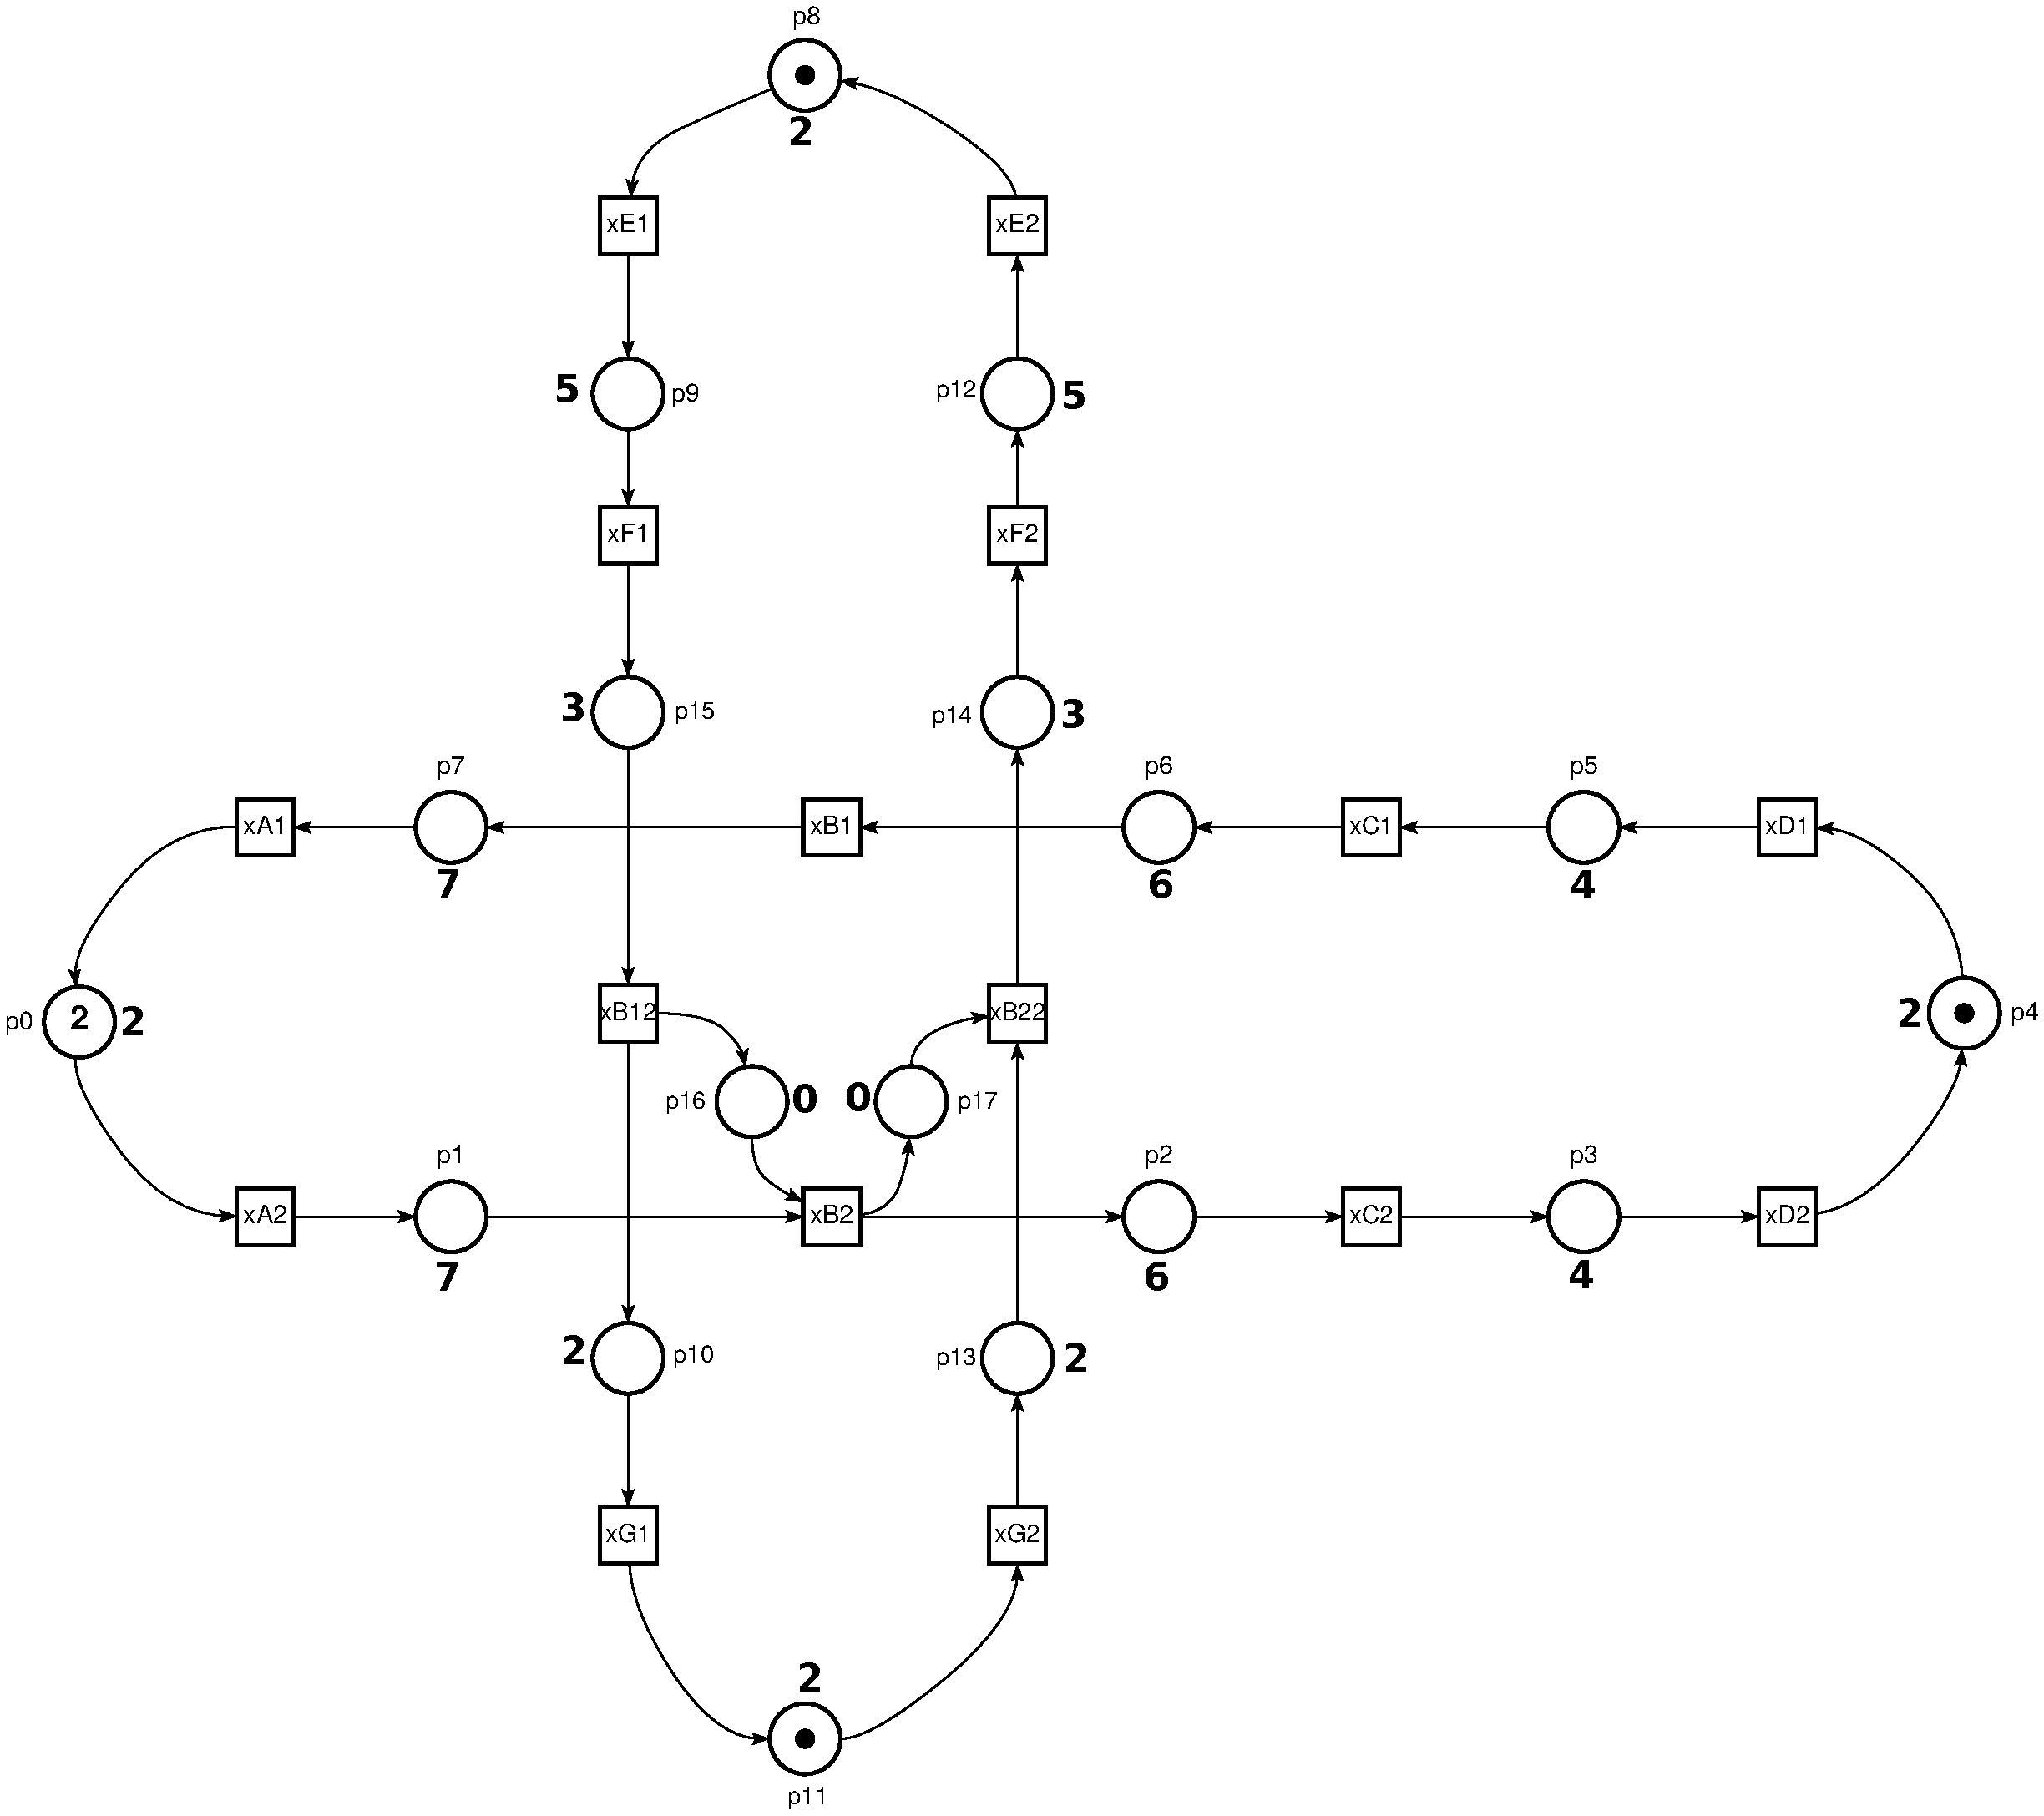
\includegraphics[width =.8 \textwidth]{./I/images/train.pdf}
\caption{\label{fig:get_train} Graphe des Événements Temporisé du réseau de transport}
\end{figure}


\begin{figure}[!ht]
\centering
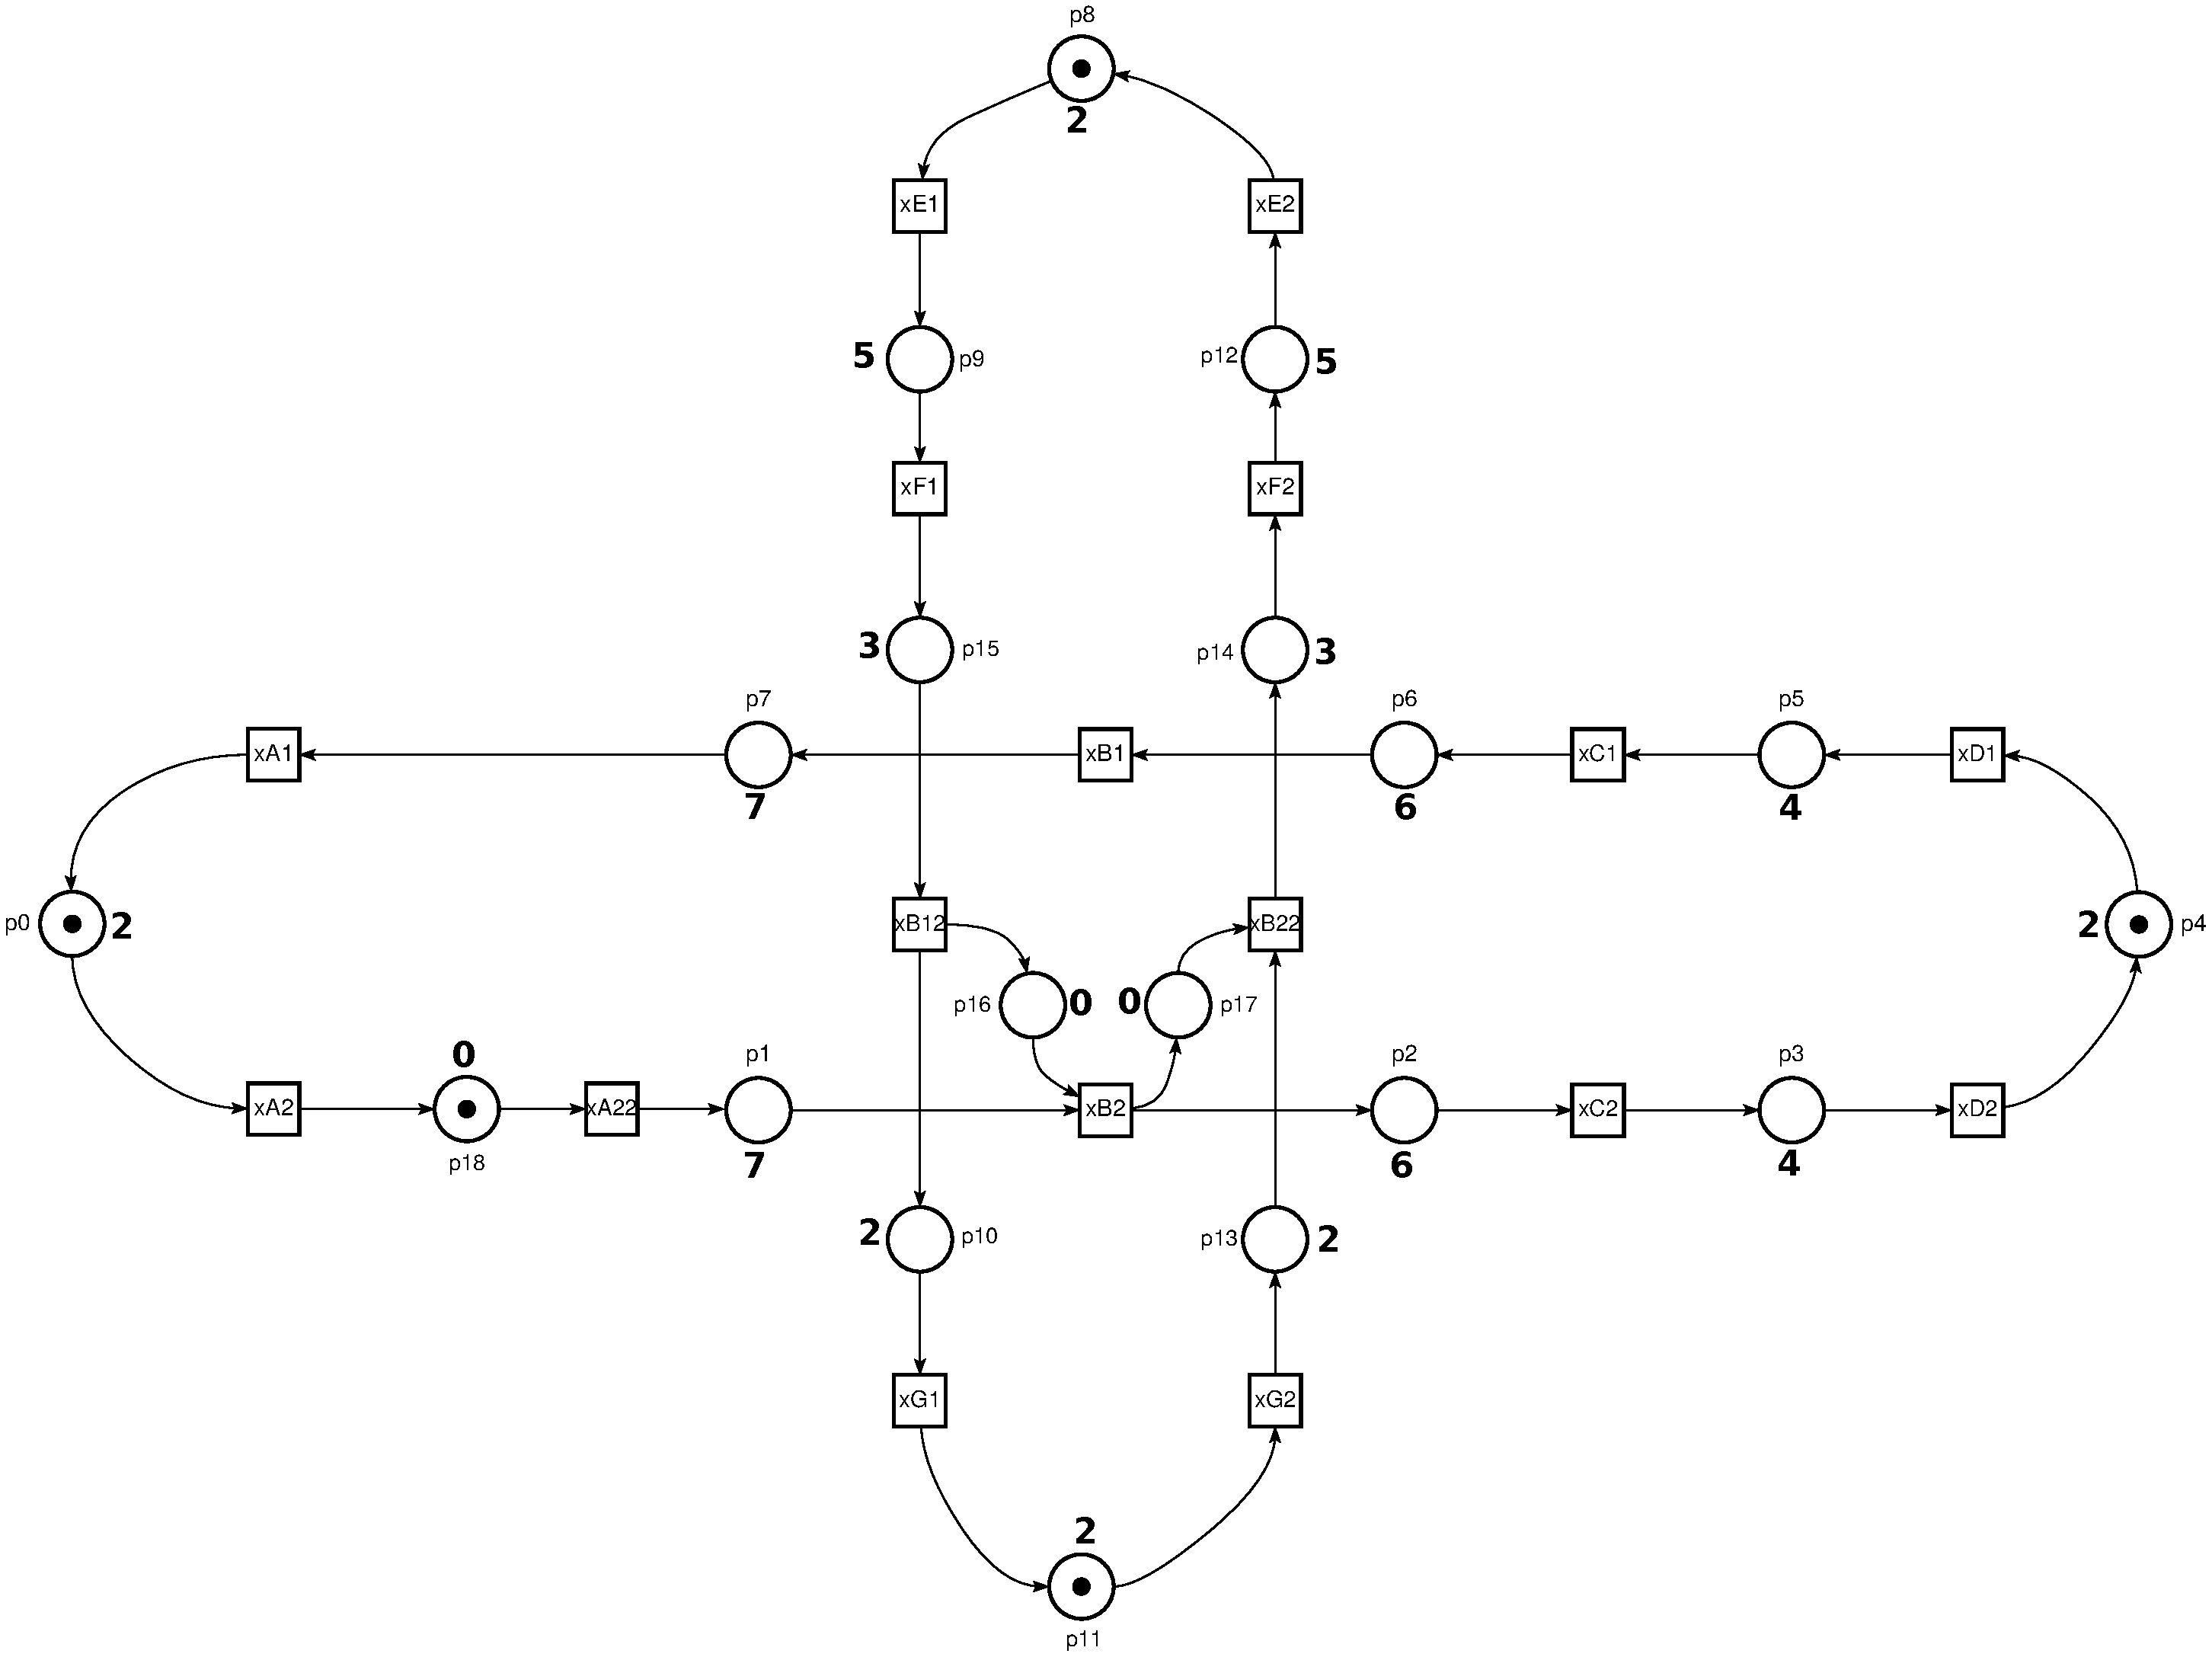
\includegraphics[width = .8\textwidth]{./I/images/train_decompose.pdf}
\caption{\label{fig:get_train_decompo} Graphe des Événements Temporisé décomposé du réseau de transport }
\end{figure}
\section{Analyse, matrice d'évolution et valeurs propres}
Nous abordons ici, dans l'ordre, la mise en représentation d'état du réseau de transport, l'analyse de réductibilité et le calcul des valeurs et vecteurs propres. 
\subsection{Représentation d'état}
Afin de réaliser la mise en représentation d'état, nous avons extrait les égalisés suivantes :
\begin{equation}
\label{equ:ee1}
\left\lbrace
\begin{array}{l c l}
x_{A1}(k) &=&	7x_{B1}(k)\\ 
x_{B1}(k) &=&	6x_{C1}(k)\\
x_{D1}(k) &=&	2x_{D2}(k-1)\\
x_{D2}(k) &=&	4x_{C2}(k)\\
x_{C2}(k) &=&	6x_{B1}(k)\\
x_{B2}(k) &=&	7x_{A2}(k) \oplus x_{B12}\\
x_{A2}(k) &=&	2x_{A1}(k-2)\\
x_{A22}(k) &=&	x_{A1}(k-1)\\
x_{E1}(k) &=&	2x_{E2}(k-1)\\
x_{F1}(k) &=&	5x_{E1}(k)\\
x_{B12}(k) &=&	3x_{F1}(k)\\
x_{G1}(k) &=&	2x_{B12}(k)\\
x_{G2}(k) &=&	2x_{G1}(k-1)\\
x_{B22}(k) &=&	2x_{G2}(k) \oplus x_{B2}(k)\\
x_{F2}(k) &=&	3x_{B22}(k)\\
x_{E2}(k) &=&	5x_{F2}(k)   \\  
\end{array}
\right.
\end{equation}
On peut remarquer que notre système est autonome, c'est-à-dire qu'il ne présente pas d'entrée ou de sortie 
dans l'espace d'état suivant, les matrices $B$ et $C$ ne sont donc pas nécessaires.
\begin{equation}
\left\lbrace
\begin{array}{lcl}
	x(k) &=& A_0 \cdot x(k) + A_1 \cdot x(k-1) + B u(k)\\
	y(k) &=& C \cdot x(k)
\end{array}
\right. \Rightarrow
\left\lbrace\begin{array}{lcl}
	x(k) &=& A \cdot x(k-1)
\end{array}\right.
\end{equation}
Ces égalités nous ont permis de créer la matrice dynamique suivante : 
\begin{equation}
A = \left(\begin{array}{ccccccccccccccccc}
.&.&.&.&19&.&.&.&.& .&.&.&.& .&.&.&. \\
.&.&.&.&12&.&.&.&.& .&.&.&.& .&.&.&. \\
.&.&.&.&6& .&.&.&.& .&.&.&.& .&.&.&. \\
.&.&.&.&2& .&.&.&.& .&.&.&.& .&.&.&. \\
.&.&.&.&.& .&.&.&19&.&.&.&.& .&.&.&20\\
.&.&.&.&.& .&.&.&15&.&.&.&.& .&.&.&16\\
.&.&.&.&.& .&.&.&9& .&.&.&.& .&.&.&10\\
.&.&.&.&.& .&.&.&2& .&.&.&.& .&.&.&.\\
0&.&.&.&.& .&.&.&.& .&.&.&.& .&.&.&. \\
.&.&.&.&.& .&.&.&.& .&.&.&.& .&.&.&2 \\
.&.&.&.&.& .&.&.&.& .&.&.&.& .&.&.&7 \\
.&.&.&.&.& .&.&.&.& .&.&.&.& .&.&.&10\\
.&.&.&.&.& .&.&.&.& .&.&.&.& .&.&.&12\\
.&.&.&.&.& .&.&.&.& .&.&.&2& .&.&.&. \\
.&.&.&.&.& .&.&.&9& .&.&.&4& .&.&.&8 \\
.&.&.&.&.& .&.&.&12&.&.&.&7& .&.&.&11\\
.&.&.&.&.& .&.&.&17&.&.&.&12&.&.&.&18
\end{array}\right)
\end{equation}
($.$ signifie $\epsilon$)
\subsection{Irréductibilité}
Maintenant que nous avons une représentation d'état de notre procédé, nous allons étudier s'il est irréductible ou non, si c'est le cas, cela signifie qu'il a une unique valeur propre (c'est une implication et non une équivalence). Une des méthodes de vérification de la propriété d'irréductibilité d'une matrice est de vérifier si elle comporte une ligne ou une colonnes d'éléments neutres ($\epsilon$).
Nous pouvons voir ici que la matrice A comporte au moins 12 colonnes d'éléments neutres, elle est donc réductible. Une des autres façon est de voir si le graphe des marquages accessible est fortement connexe ou non. Si il n'est, elle est irréductible. Figure \ref{fig:gma_train}, on peut voir que ce n'est pas le cas les états 2, 3, 4, 6, 7, 8, 10, 11, 12, 14, 15 et 16 sont des états puits.
\begin{figure}[!ht]
\centering
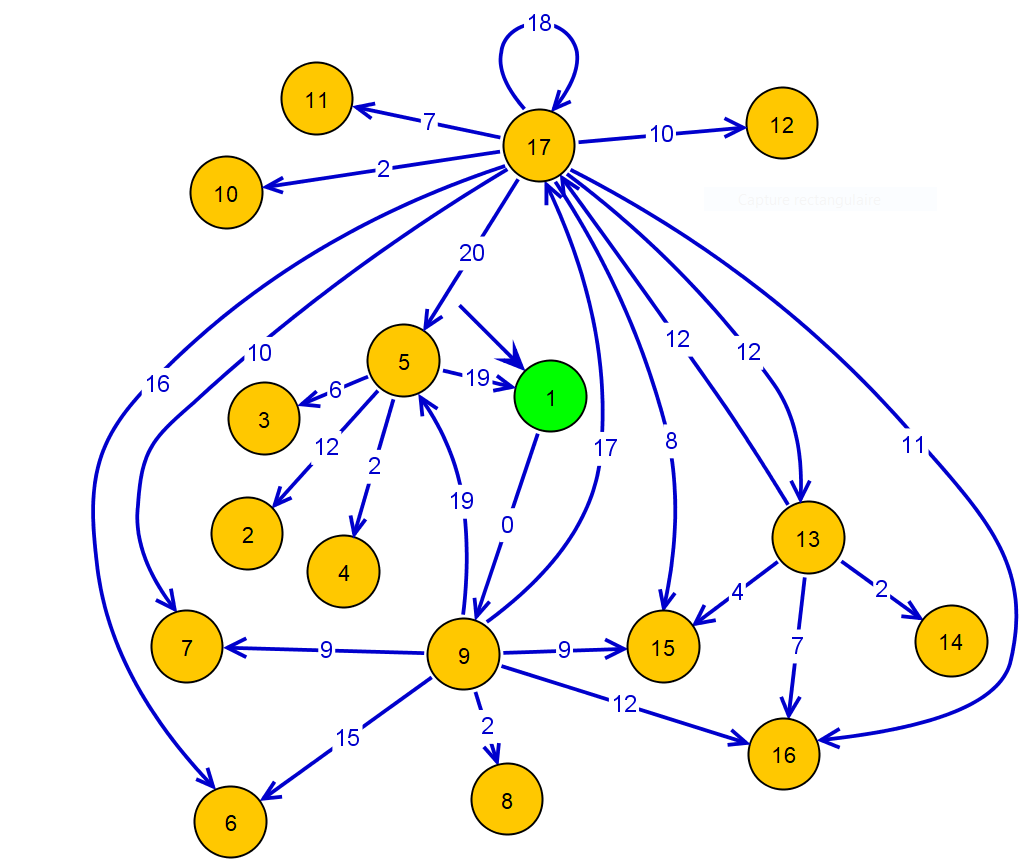
\includegraphics[width = .4\textwidth]{./I/images/GMA.png}
\caption{\label{fig:gma_train} Graphe des Marquages accessibles de $A$}
\end{figure}
\subsection{Valeur propre}
Nous avons calculé la valeur propre à l'aide de ScicosLab, elle est unique est vaux 18. Cela veut dire que le cycle interne du système est de 18 événements une fois le régime permanent établi.
\subsection{Vecteur propre}
Comme précédemment, nous avons utilité ScicosLab pour calculer le vecteur propre de $A$.
\begin{equation}
vecteur_{propre} = 
\left[
\begin{array}{ccccccccccccccccc}
21 & 14 & 8 & 4 & 20 & 16 & 10 & -13 & 3 & 2 & 7 & 10 & 12 & -4 & 8 & 11 & 18	
\end{array} \right]^T
\end{equation}

\section{Commande des conditions initiales}
Dans cette partie, nous allons étudier l'évolution des trains et étudier les temps d'arrivés des trains aux différentes gares. 
Dans un premier temps nous créerons le vecteur d'état initiaux à partir de contraintes spécifiés dans l'énoncé, nous calculerons les temps d'évolutions des trains à partir de ces conditions initiales. Nous étudierons également des contraintes de synchronisation, identifierons l'amélioration du système par ajout d'un train et finalement nous évaluerons l'impact d'une modification du réseau.
\subsection{Vecteur d'état initiaux}
Nous avons les contraintes suivantes : 
\begin{enumerate}
\item Un train part de la station \textbf{D} à la date \textbf{1};%1
\item Un train part de la station \textbf{A} à la date \textbf{3};%2
\item Un train part de la station \textbf{E} à la date \textbf{3};%3
\item Un train part de la station \textbf{A} à la date \textbf{7};%4
\item Un train part de la station \textbf{G} à la date \textbf{8}.%5
\end{enumerate}
A partir de ces contraintes, nous avons calculé le vecteur initial suivant: 
\begin{equation}
X0 = 
\left[
\begin{array}{ccccccccccccccccc}
18  &11  &5   &1   &21  &17  &11  &3   &5   &3   &8   &11  &13  &8   &11  &14  &19 
\end{array} \right]^T
\end{equation}
Pour ce calcul, nous avons dans un premier temps placé, les temps de départ de chaque trains aux indices corresponds au départ de la gare concernée : 
\begin{description}

\item[Contrainte 1 :] $X0(D1) = 1$; 
\item[Contrainte 2 :] $X0(A2) = 3$; 
\item[Contrainte 3 :] $X0(E1) = 3$; 
\item[Contrainte 4 :] $X0(A22) = 5$ (car 2 u.t déjà consommée en $p0$) ; 
\item[Contrainte 5 :] $X0(G2) = 8$. 
\end{description}
A partir de ces données, nous avons calculé les valeurs des autres états en étudiant le GET.


\subsection{Calculs des 10 premiers trains arrivants en gare C et venant de la gare B}
Afin d'effectuer l'analyse demandé et pour avoir une vision globale des temps d'arrivées dans les autres gares, nous avons généré les 10 premiers temps d'arrivées de l'ensemble du réseau. (La petite taille du réseau rendant cette génération possible en terme de temps de calcul.)

Pour cela, nous avons initialisé un vecteur de dimension : $\mathbb{R}^{ \text{\emph{nombre d'états}} \times \text{\emph{nombre de temps d'arrivé souhaité}}}$.\\
Ensuite, nous avons initialisé la première colonne avec le vecteur d'état initiaux et les avons calculer les suivantes dans une boucle en effectuant le calcul suivant : 
\begin{eqnarray}
\forall i \in \left\lbrace 2, ..., 10\right\rbrace | X_1 = X0 ,&    X_{i}&=A*X_{(i-1)}\\
\Leftrightarrow&&\\
\forall i \in \left\lbrace 1, ..., 10\right\rbrace ,&    X_{i}&=X_0*A^i
\end{eqnarray}

Les dates de départs correspondants aux trains arrivants en C et venant de B sont ceux  de la ligne 7 de $X$ :
\begin{equation}
L_7(X)= \begin{bmatrix} 11&29&47&65&83&101&119&137&155&173 \end{bmatrix}
\end{equation}


Voici une représentation graphique figure \ref{fig:temps_arrivee} (effectué à l'aide de Matlab) où nous pouvons voir que les temps de départs se stabilise rapidement car la pente est constante au bout d'un certain nombre d'événement.
\begin{figure}[!ht]
\centering
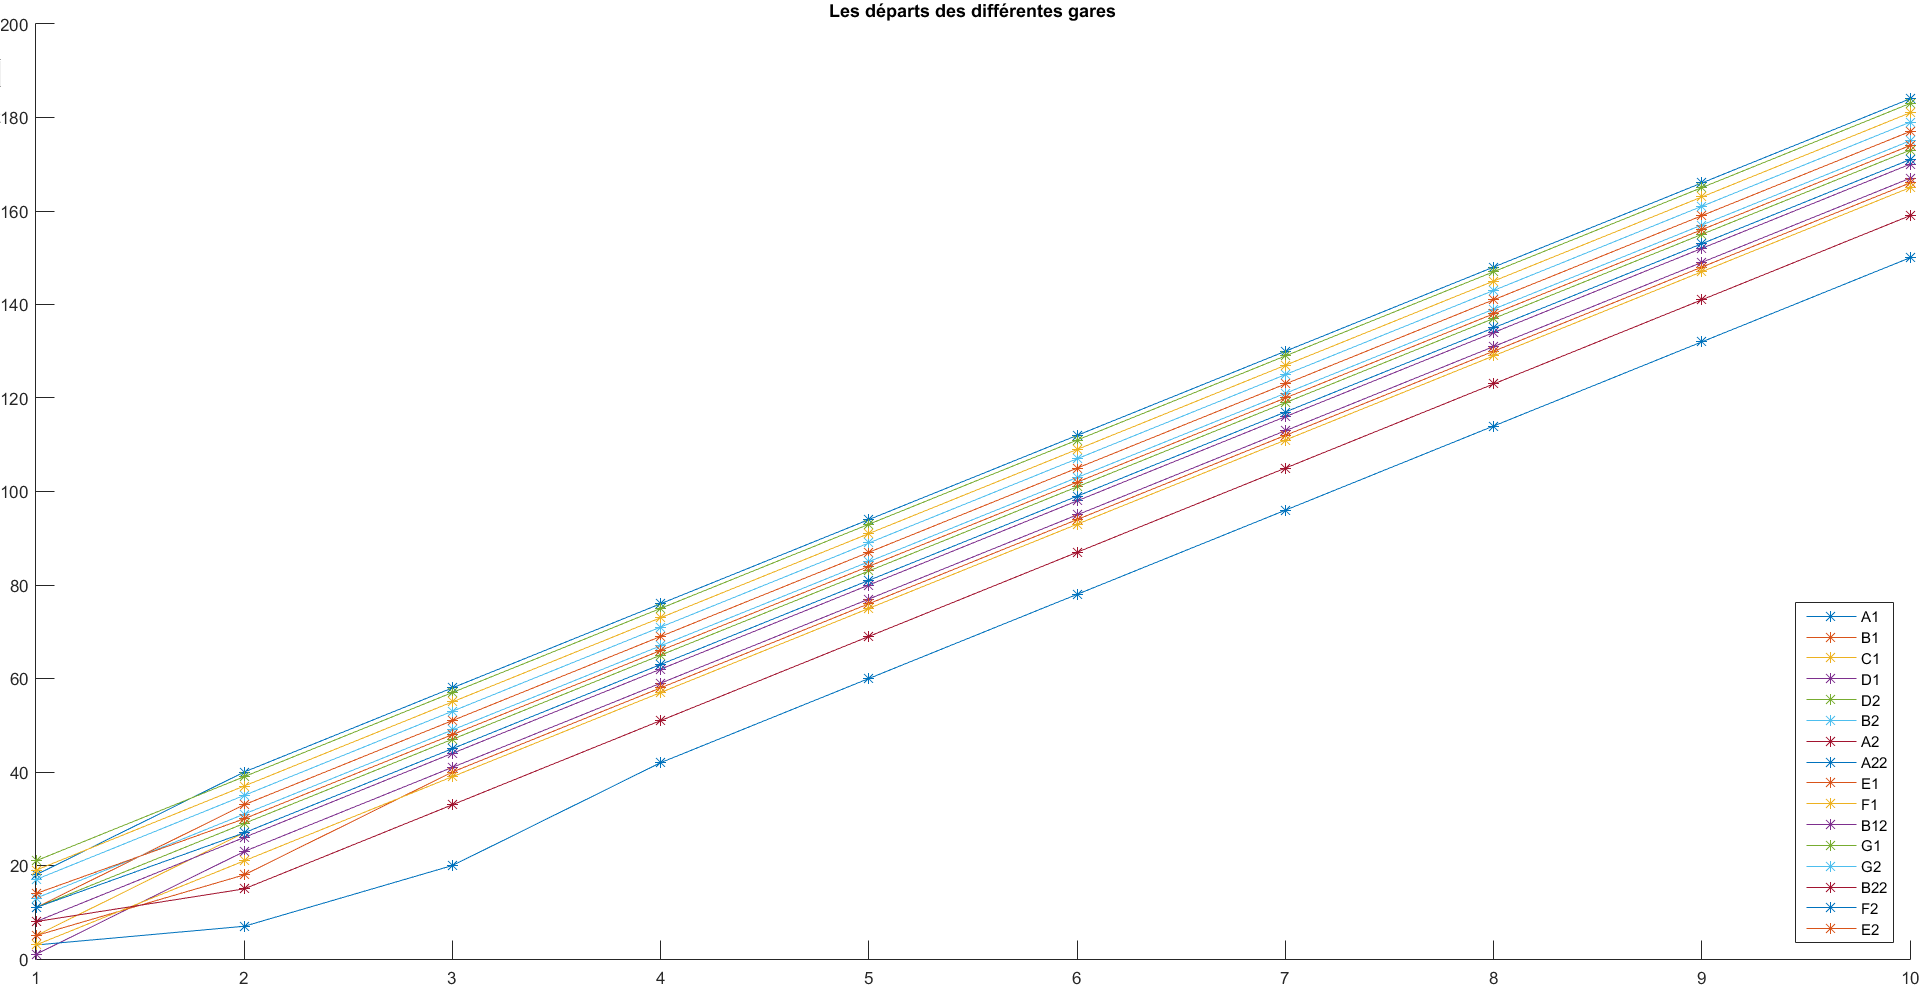
\includegraphics[width = .7\textwidth]{./I/images/temps_departs.png}
\caption{\label{fig:temps_arrivee} Temps de départ des trains dans les différentes gares}
\end{figure}


Nous avons décidé d'étudier la différence suivante $\Delta_{cy} = X_i - X_{i-1}$ où $i = \left\lbrace 1,...,9\right\rbrace$. Cela nous a permis de calculer le nombre d'événement nécessaire à l'entrée dans le cycle périodique.
\begin{equation}
\Delta_{cy} = 
\left(
\begin{array}{cc cc cc cc cc}
22 & 18 & 18 & 18 & 18 & 18 & 18 & 18 & 18 \\
22 & 18 & 18 & 18 & 18 & 18 & 18 & 18 & 18 \\
22 & 18 & 18 & 18 & 18 & 18 & 18 & 18 & 18 \\
22 & 18 & 18 & 18 & 18 & 18 & 18 & 18 & 18 \\
18 & 18 & 18 & 18 & 18 & 18 & 18 & 18 & 18 \\
18 & 18 & 18 & 18 & 18 & 18 & 18 & 18 & 18 \\
18 & 18 & 18 & 18 & 18 & 18 & 18 & 18 & 18 \\
4 &  13 & 22 & 18 & 18 & 18 & 18 & 18 & 18 \\
13 & 22 & 18 & 18 & 18 & 18 & 18 & 18 & 18 \\
18 & 18 & 18 & 18 & 18 & 18 & 18 & 18 & 18 \\
18 & 18 & 18 & 18 & 18 & 18 & 18 & 18 & 18 \\
18 & 18 & 18 & 18 & 18 & 18 & 18 & 18 & 18 \\
18 & 18 & 18 & 18 & 18 & 18 & 18 & 18 & 18 \\
7 &  18 & 18 & 18 & 18 & 18 & 18 & 18 & 18 \\
16 & 18 & 18 & 18 & 18 & 18 & 18 & 18 & 18 \\
16 & 18 & 18 & 18 & 18 & 18 & 18 & 18 & 18 \\
18 & 18 & 18 & 18 & 18 & 18 & 18 & 18 & 18 
\end{array}
\right)
\end{equation}
Nous pouvons constater qu'à partir du  5\ieme{} départs, tous les trains partent toutes les 18 u.t, cela correspond à la valeur propre et cela permet de renforcer la validité de nos calculs, de plus nous pouvions le voir graphiquement sur la figure \ref{fig:temps_arrivee}.

\subsection{Temps inter-arrivées identiques}
Afin d'avoir des temps d'inter-arrivées tous identiques, nous avons refais les opérations nécessaire au calcul de $X$ avec $X_1=vecteur_{propre}$.

De cette façon, nous avons des temps inter-arrivées identiques et qui valent la valeur propre du système soit $18$. Nous l'avons recalculé $\Delta_{cy}$ et toutes les différences de temps valent $18$.


\subsection{Ajout d'un train}
Nous devons ajouter un train afin d'accélérer le temps de cycle. Dans un premier temps, nous allons identifier le cycle a accélérer pour accélérer le réseau, ensuite nous ajouterons un train à la bonne gare et finalement nous évaluerons l'amélioration.

La valeur propre étant le temps du plus long cycle, il faut que l'on trouve le/les sous-cycle(s) qui correspond à cette durée. Cela correspond à, au départ d'un train d'un terminus, le nombre d'unité de temps qu'il faut attendre avant qu'un autre train arrive dans ce même terminus. Sur le GET, cela revient au prochain au temps écoulé entre deux tirs d'une même transition.
Nous avons trouvé que c'est le trajet E-B  $\rightarrow$  B-E qui prend le plus de temps. Nous allons donc ajouter un train sur la gare E. 
Nous ajoutons donc un jeton en $p8$ sur la figure \ref{fig:get_train}. Cela donne, une fois décomposé de la même façon que la figure \ref{fig:get_train_decompo}, la figure \ref{fig:get_train_decompo2}.

\begin{figure}[!ht]
\centering
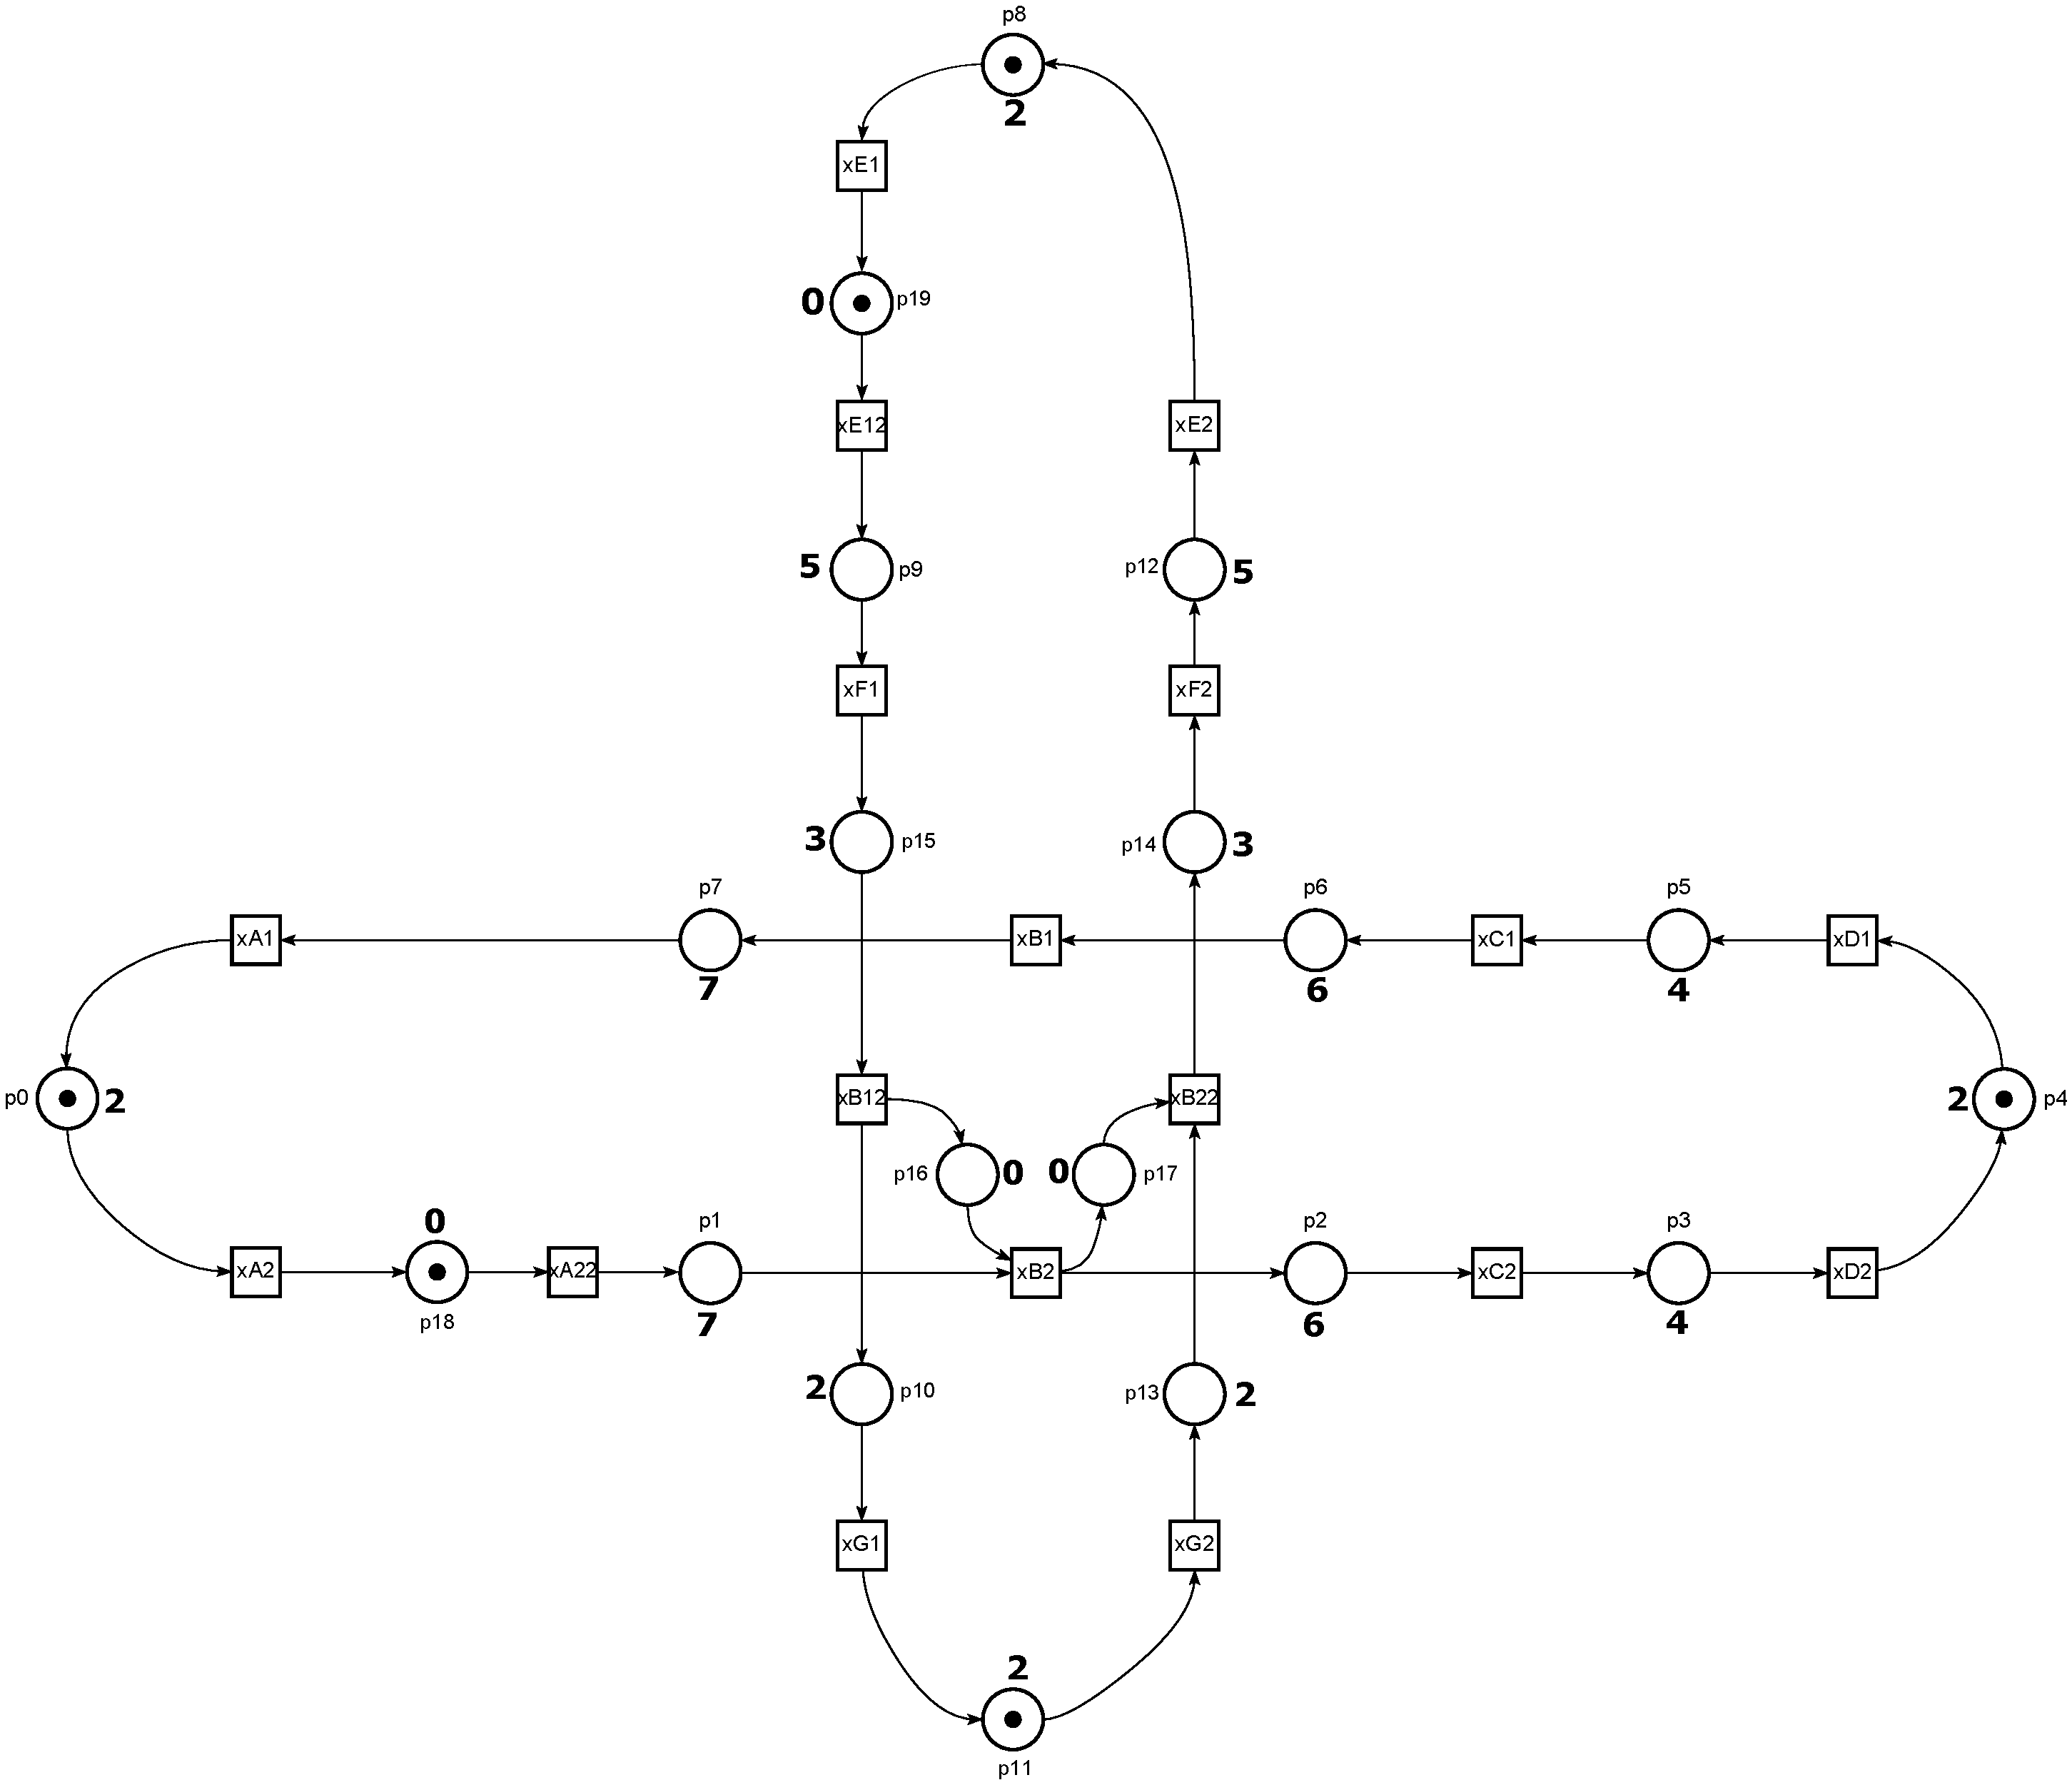
\includegraphics[width = .8\textwidth]{./I/images/train_decompose2.pdf}
\caption{\label{fig:get_train_decompo2} Graphe des Événements Temporisé décomposé du réseau de transport avec l'ajout d'un nouveau train.}
\end{figure}

Afin de recalculer une nouvelle matrice dynamique $A2$, nous avons redéfinis les équations d'états de la même façon que précédemment (équation \ref{equ:ee1}). 

Voici les nouvelles équations d'état :
\begin{equation}
\label{equ:ee1}
\left\lbrace
\begin{array}{l c l}
x_{A1}(k) &=&	7x_{B1}(k)\\ 
x_{B1}(k) &=&	6x_{C1}(k)\\
x_{D1}(k) &=&	2x_{D2}(k-1)\\
x_{D2}(k) &=&	4x_{C2}(k)\\
x_{C2}(k) &=&	6x_{B1}(k)\\
x_{B2}(k) &=&	7x_{A2}(k) \oplus x_{B12}\\
x_{A2}(k) &=&	2x_{A1}(k-2)\\
x_{A22}(k) &=&	x_{A1}(k-1)\\
x_{E1}(k) &=&	2x_{E2}(k-1)\\
x_{F1}(k) &=&	5x_{E12}(k)\\
x_{B12}(k) &=&	3x_{F1}(k)\\
x_{G1}(k) &=&	2x_{B12}(k)\\
x_{G2}(k) &=&	2x_{G1}(k-1)\\
x_{B22}(k) &=&	2x_{G2}(k) \oplus x_{B2}(k)\\
x_{F2}(k) &=&	3x_{B22}(k)\\
x_{E2}(k) &=&	5x_{F2}(k)   \\  
x_{E12}(k) &=&	x_{E1}(k-1)   \\  
\end{array}
\right.
\end{equation}
La définition de $x_{F1}(k)$ est maintenant exprimée à partir de $x_{E12}(k)$ et celle de $x_{E12}(k)$ à partir de $x_{E1}(k)$, le reste est identique.
La dimension de $A2$ est donc agrandie d'un état par rapport a celle de $A$.


Voici la matrice dynamique $A2$ de notre système avec un train de plus :




